\section*{Entrando en un agujero negro}
\underline{Surface Gravity ($\kappa$)}: 
\begin{align*}
    &\text{Aceleración que debe tener un observador estático en el horizonte de eventos para}\\
    &\text{no caer, vista por un observador en el infinito.}\\
    &\text{En agujero negro de Schwarzschild: } \kappa= \frac{1}{2} \; \xrightarrow{\text{S.I.}}\; \kappa= \frac{c^4}{4GM}
\end{align*}
\underline{Distancia propia}:
\begin{align*}
    &\text{Distancia física que se mediría en un cierto espacio-tiempo:}\\
    &1. \text{ Parametrizamos la curva que queremos medir.}\\
    &2. \text{ Diferencia con respecto al parámetro escogido.}\\
    &3. \text{ Sustituye en $ds^2$ e iguala a $d\rho^2$.}\\
    &4. \text{ Integra a ambos lados para obtener $\rho\equiv$ distancia propia.}
\end{align*}
\underline{Métrica en las cercanías del horizonte de eventos de Schwarzschild}: 
\begin{align*}
    &ds^2 \approx - \rho^2 \,d\varrho^2+ d\rho ^2 + d\Omega^2\; \; \; d\Omega^2=d\theta^2 + \sin^2 \theta\,\,d\phi^2 \; \; \; \; \rho\approx \sqrt{\frac{2}{\kappa}}\,\sqrt{r-1}\; \; \; \; \varrho\equiv \kappa \,t\\
    &\text{La métrica se comporta como la métrica de Rindler} \Rightarrow \Gamma^\varrho_{\rho \varrho}= \frac{1}{\rho}\; \; \; \; \Gamma^\rho_{\varrho \varrho}= \rho \\
    &\text{Para un observador estático: }\underline{u}=u^0e_0= \frac{1}{\rho}e_\varrho\; \; \; \underline{a}=\frac{1}{\rho}e_\rho=\kappa e_1\\
    &\text{Para observadores en caída libre, sus trayectorias espacio-temporales serán líneas}\\
    &\text{verticales (oblícuas si tienen velocidad inicial) que intersecarán con la línea $x=ct$,}\\
    &\text{correspondiente al horizonte de eventos.}
\end{align*}
\underline{Métrica dentro del agujero negro de Schwarzschild, cerca del horizonte de eventos}:
\begin{align*}
    &ds^2 \approx - \frac{1}{1-r}\,dr^2 + (1-r)\,dt^2 +d\Omega^2\; \; \; \;\; 0<< r< 1\; \Rightarrow\text{Cambia el signo de las}\\
    &\text{dos primeras coordenadas: $t$ se comporta como coordenada tipo ``espacio", y $r$ se}\\
    &\text{comporta como coordenada tipo ``tiempo". Ocurrirá también para $0<r<1$.}\\
    &\text{Cambio de coordenadas: }ds^2 \approx -du^2+ u^2 dv^2+d\Omega^2\;\;\;\; u\equiv2\sqrt{1-r}\; \;\; \; v\equiv t/2\\
    &\text{Cambio de coordenadas: }ds^2\approx -dT^2 +dX^2+d\Omega^2 \; \; \; \; T\equiv u\cosh v\; \; \; \; X\equiv u \sinh v \\
    &\text{Un observador estático tendrá $t$ cte $\Rightarrow$ será visto como observador incercial según}\\
    &\text{el observador en caída libre (será representado con líneas rectas oblícuas).}\\
    &\text{Los instantes de tiempo  vienen dados por $r$ cte (serán representados por hipérbolas).}
\end{align*}
\hspace{60pt}
\begin{minipage}{0.48\linewidth}
    \centering
    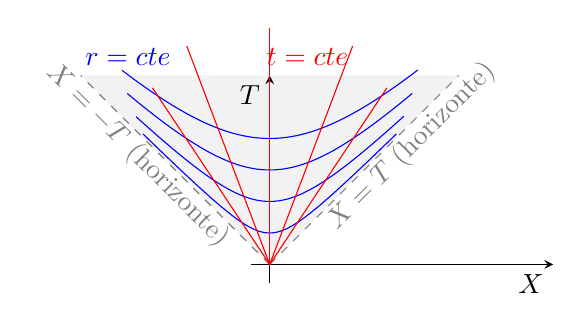
\begin{tikzpicture}[scale=1.2,>=stealth]

% Cuña de Rindler (girada 90º)
\fill[gray!10] (0,0) -- (-2,2) -- (2,2) -- cycle;

% Ejes (se mantienen)
\draw[->] (-0.2,0) -- (3,0) node[below left] {$X$};
\draw[->] (0,-0.2) -- (0,2) node[below left] {$T$};

% Cono de luz (girado)
\draw[dashed, gray] (0,0) -- (-2,2);  \node[rotate=-45,gray] at (-1.4,1.15) {$X=-T$ (horizonte)};
\draw[dashed, gray] (0,0) -- (2,2) node[rotate=45] at (1.5,1.25){$X=T$ (horizonte)};


% Hipérbolas (giradas)
\foreach \xi in {1/3}{
    \draw[blue, domain=-2.1:2.1, samples=200, variable=\eta] 
        plot ({-\xi*sinh(\eta)}, {\xi*cosh(\eta)});
}
\foreach \xi in {2/3}{
    \draw[blue, domain=-1.5:1.5, samples=200, variable=\eta] 
        plot ({-\xi*sinh(\eta)}, {\xi*cosh(\eta)});
}
\foreach \xi in {3/3}{
    \draw[blue, domain=-1.2:1.2, samples=200, variable=\eta] 
        plot ({-\xi*sinh(\eta)}, {\xi*cosh(\eta)});
}
\foreach \xi in {4/3}{
    \draw[blue, domain=-1:1, samples=200, variable=\eta] 
        plot ({-\xi*sinh(\eta)}, {\xi*cosh(\eta)});
}

% Rectas eta = const (giradas)
\foreach \eta in {-0.8,-0.4,0,0.4,0.8}{
    \draw[red] (0,0) -- ({-2.5*tanh(\eta)/cosh(\eta)}, {2.5/cosh(\eta)});
}

% Etiquetas (reubicadas un poco)
\node[blue] at (-1.5,2.2) {$r = \text{cte}$};
\node[red] at (0.4,2.2) {$t = \text{cte}$};

\end{tikzpicture}
\end{minipage}

\underline{Métrica dentro del agujero negro de Schwarzschild}:
\begin{align*}
     &\dashv \text{ Métrica de Kruskal-Szekeres: } ds^2=\frac{4}{r}e^{-r}(-dT^2 + dX^2)+r^2\,d\Omega^2 \; \; \; \; 0<r<1.\\
     &T\equiv  \sqrt{1-r}\, e^{r/2}\cosh\frac{t}{2} \; \; \; \; X\equiv  \sqrt{1-r}\, e^{r/2}\sinh\frac{t}{2}\; \; \; \; T^2-X^2=(1-r)\, e^r
\end{align*}


\hspace{60pt}
\begin{minipage}{0.48\linewidth}
\centering
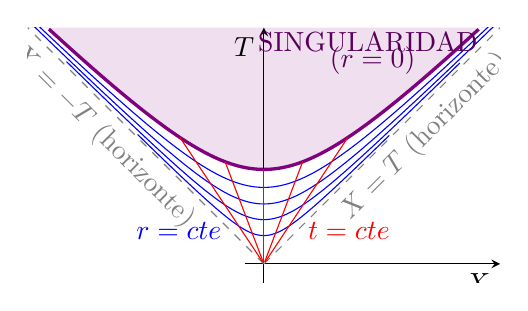
\begin{tikzpicture}[scale=1.2,>=stealth]
  %----- Parámetros de la ventana -----
  \def\Xmax{2.5}
  \def\Tmax{2.5}
  \clip (-\Xmax,-0.2) rectangle (\Xmax,\Tmax);


  %----- Zona de la singularidad: T^2 - X^2 \ge 1 (r=0) -----
  % Rellenamos por encima de T = sqrt(1+X^2) dentro del marco.
  \begin{scope}
    \clip (-\Xmax,0) rectangle (\Xmax,\Tmax);
    \fill[violet!25, opacity=0.5]
      plot[domain=-\Xmax:\Xmax,samples=400,variable=\x]
        ({\x},{sqrt(1+\x*\x)})
      -- (\Xmax,\Tmax) -- (-\Xmax,\Tmax) -- cycle;
  \end{scope}
  % Borde de la singularidad (r=0)
  \draw[violet, very thick, domain=-\Xmax+0.225:\Xmax-0.225, samples=400, variable=\x]
    plot ({\x},{sqrt(1+\x*\x)});

  %----- Ejes -----
  \draw[->] (-0.2,0) -- (\Xmax,0) node[below left] {$X$};
  \draw[->] (0,-0.2) -- (0,\Tmax) node[below left] {$T$};

  %----- Horizontes: X= \pm T (T^2-X^2=0) -----
  \draw[dashed,gray] (0,0) -- (\Xmax,\Xmax);
  \draw[dashed,gray] (0,0) -- (-\Xmax,\Xmax);
  \node[rotate=45,gray] at (1.7,1.35) {$X=T$ (horizonte)};
  \node[rotate=-45,gray] at (-1.7,1.35) {$X=-T$ (horizonte)};

  %----- Curvas r = cte (hipérbolas T^2 - X^2 = (1-r)e^{r}) -----
  % Elegimos r en (0,1) para permanecer dentro de T^2-X^2 \le 1.
  \foreach \r in {0.2,0.4,0.6,0.8} {
    \pgfmathsetmacro{\A}{sqrt(1-\r)*exp(-\r/2.0)} % A = sqrt(1-r) e^{-r/2}
    \draw[blue, domain=-2.2:2.2, samples=500, variable=\eta]
      plot ({\A*sinh(\eta)}, {\A*cosh(\eta)});
  }

  %----- Curvas t = cte (rectas desde el origen: X/T = tanh(t/2)) -----
  % Parametrizamos con r \in [0,1]: B(r)=sqrt(1-r)e^{-r/2}
  \foreach \t in {-1.6,-0.8,0,0.8,1.6} {
    \pgfmathsetmacro{\halfT}{\t/2.0}
    \draw[red, domain=0:1, samples=300, variable=\rr]
      plot (
        { sqrt(1-\rr)*exp(-\rr/2.0)*sinh(\halfT) },
        { sqrt(1-\rr)*exp(-\rr/2.0)*cosh(\halfT) }
      );
  }

  %----- Etiquetas -----
  \node[blue] at (-0.9,0.35) {$r=\text{cte}$};
  \node[red]  at (0.9,0.35) {$t=\text{cte}$};
  \node[violet!70!black] at (1.1,2.35) {SINGULARIDAD};
  \node[violet!70!black] at (1.15,2.15) {($r=0$)};

\end{tikzpicture}
\end{minipage}
\\
\vspace{5pt}
\underline{Generalización de las coordenadas de Kruskal-Szekeres en las 4 zonas del espacio-tiempo}:
\begin{align*}
    &\text{Podemos generalizar las coordenadas obtenidas previamente para la zona II (dentro}\\
    &\text{del horizonte de eventos) a la zona I (fuera del horizonte de eventos) y a las zonas}\\
    &\text{III y IV (artificios mátemáticos). La métrica es la de Kruskal-Szekeres en toda zona.} 
\end{align*}
\[
\resizebox{0.33\textwidth}{!}{$
\begin{array}{c|c|c|c}
\text{Zona I} & 
\text{Zona II} & 
\text{Zona III} & 
\text{Zona IV} \\
\hline
\rule{0pt}{2.4em} 
\begin{aligned}
T &= \sqrt{r-1}\, e^{r/2} \sinh\frac{t}{2}\\
X &= \sqrt{r-1}\, e^{r/2}  \cosh\frac{t}{2}
\end{aligned}
&
\begin{aligned}
T &= \sqrt{1-r}\,  e^{r/2}  \cosh\frac{t}{2} \\
X &= \sqrt{1-r}\,  e^{r/2}  \sinh\frac{t}{2}
\end{aligned}
&
\begin{aligned}
T &= -\sqrt{r-1}\, e^{r/2}  \sinh\frac{t}{2} \\
X &= -\sqrt{r-1}\,  e^{r/2} \cosh\frac{t}{2}
\end{aligned}
&
\begin{aligned}
T &= -\sqrt{1-r}\,  e^{r/2}  \frac{t}{2} \\
X &= -\sqrt{1-r}\,  e^{r/2} \frac{t}{2}
\end{aligned}
\\
\end{array}
$}
\]
\underline{Diagrama de las 4 zonas del espacio-tiempo}:
\begin{center}
    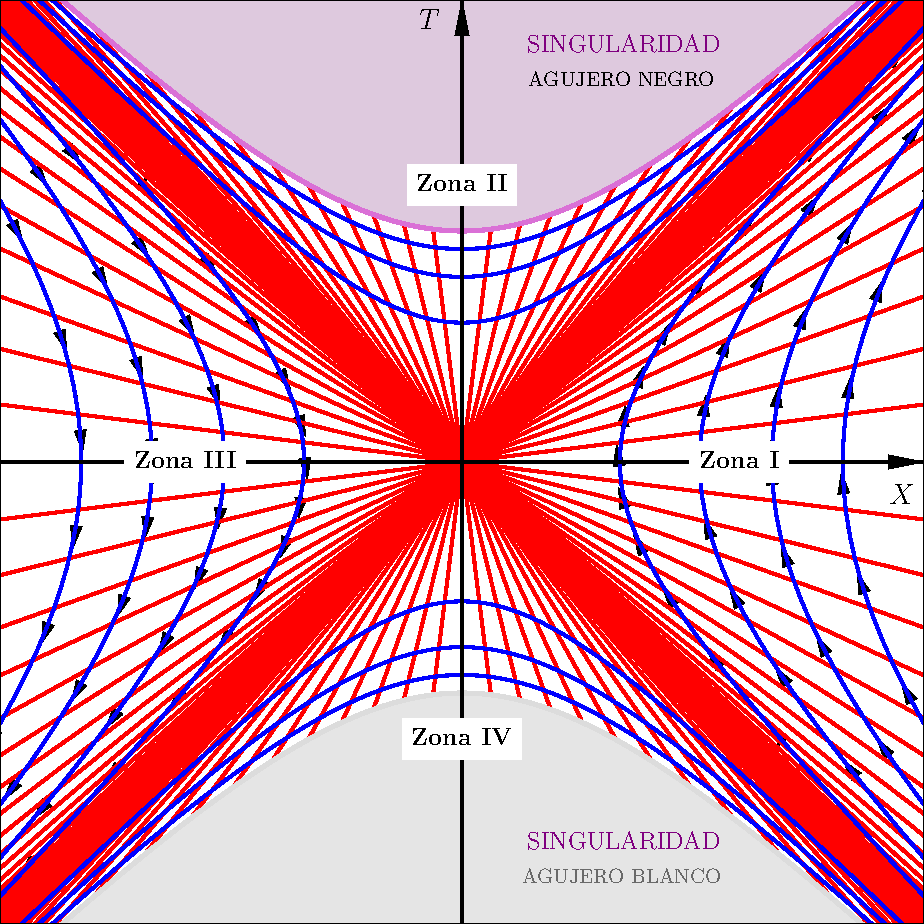
\includegraphics[height=200pt]{sections/F1_diagrama.pdf}
\end{center}
\begin{align*}
    &\text{La relación }T^2-X^2=(1-r)\, e^r \text{ es válida en las 4 zonas, permitiendo determinar}\\
    &\text{la coordenada $r$ correspondiente al par $(T,X)$. Sin embargo, para un mismo valor}\\
    &\text{de $r$ pueden corresponder puntos con $X>0$ o $X<0$. Para conseguir una relación }\\
    &\text{inequívoca, se toma el tiempo  coordenado $t<0$ en la zona III, de acuerdo con las}\\
    &\text{flechas del diagrama.}\\
    &\text{No obstante, hay que recordar que el tiempo coordenado $t$ es una \textit{etiqueta} para}\\
    &\text{describir el espacio-tiempo. Lo físicamente relevante es el tiempo propio medido}\\
    &\text{por un observador, que siempre avanza hacia el futuro y nunca puede decrecer a lo}\\
    &\text{a lo largo de su trayectoria.}
\end{align*}
\underline{Métrica de Einstein-Rose}
\begin{align*}
    &\dashv\;  ds^2=-\frac{u^2}{4+u^2}dt^2 + \frac{4+u^2}{4}du^2 + \left(1+\frac{u^2}{4}\right)^2 d\Omega^2\; \; \;\; r=1+\frac{u^2}{4} \in[1,\infty)\\
    &\text{Cambio de coordenadas (tipo Kruskal): }ds^2=\frac{4}{1+\frac{u^2}{4}}e^{-(1+\frac{u^2}{4})}(-dT^2+dX^2)\\
    &T=\frac{u}{2}e^{\frac{1}{2}+\frac{u^2}{8}}\sinh\frac{t}{2}\; \; \; \; X=\frac{u}{2}e^{\frac{1}{2}+\frac{u^2}{8}}\cosh\frac{t}{2}\; \; \; \; d\Omega\equiv \text{cte}\; \; \;  X^2-T^2=\frac{u^2}{4}e^{1+\frac{u^2}{4}}\\
    &\text{$u=0\rightarrow $ horizonte de eventos}\; \; \; u>0\rightarrow\text{ zona I}\; \;\; u<0 \rightarrow\text{ zona III}\\
    &\text{No existe ningún posible valor de $u$ que nos sitúe en la zona II o zona IV.}\\
    &\frac{dt}{d\tau}=\frac{4+u^2}{u^2} \; \; \; \; \frac{du}{d\tau}=\frac{-4}{u\sqrt{4+u^2}}\; \; \; v_{\text{obs lejano}}=\frac{du}{dt}=-\frac{4u}{(4+u^2)^{3/2}}\\
    &\text{Para un observador estático: } (dt)_{\text{est}} =\sqrt{\frac{u^2}{4+u^2}} \, dt\;\; \; \; (du)_{\text{est}}=\sqrt{\frac{4+u^2}{4}}\, du\\
    &v_{\text{obs est}}=\frac{(du)_{\text{est}}}{(dt)_{\text{est}}} = \frac{2}{\sqrt{4+u^2}}\xrightarrow{u=0} 1\xrightarrow{\text{S.I.}}c \; \; (\text{imposible pasar de zona I a III)}
    \end{align*}